\clearpage
\section{Technische Grundlagen Zigbee}\label{sec:TechnischeGrundlagenZigbee}

\subsection{Netzaufbau und Topologie}\label{subsec:NetzaufbauundTopologie}
\todo[inline]{Welchen Aufbau? Welche Art von Mesh? Welche Nodetypen gibt es? Welche typischen Eigenschaften besitzt das Protokoll?}

\begin{figure}[h]
	\centering
	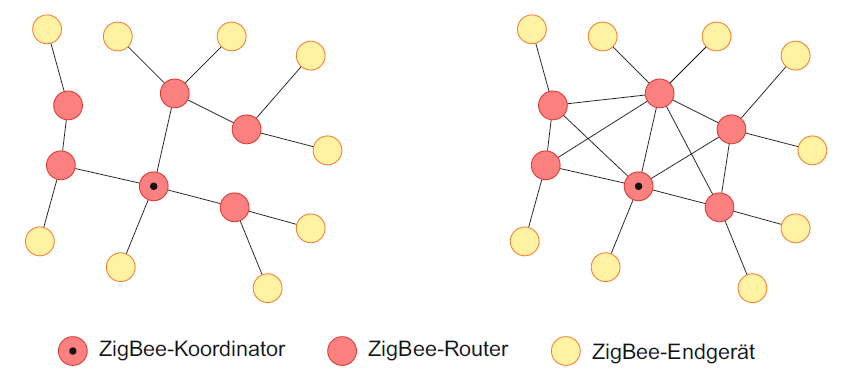
\includegraphics[width=0.8\textwidth]{Zigbee_Netztopologie.png}
	\caption{Netzwerktopologien Zigbee}
	\label{fig:NetzwerktopologienZigbee}
\end{figure}

\subsubsection{Nodetypen}\label{subsubsec:Nodetypen}
\paragraph{Zigbee Coordinator}\label{para:ZigbeeCoordinator}

\paragraph{Zigbee Router}\label{para:ZigbeeRouter}

\paragraph{Zigbee End Device}\label{para:ZigbeeEndDevice}





\subsection{Zigbee Protokoll Stack}\label{subsec:ZigbeeProtokollStack}
\todo[inline]{Erläuterung des Protokoll Stacks. Möglichst viel Grafiken und nur so viel als nötig Prosa.}

\begin{figure}[h]
	\centering
	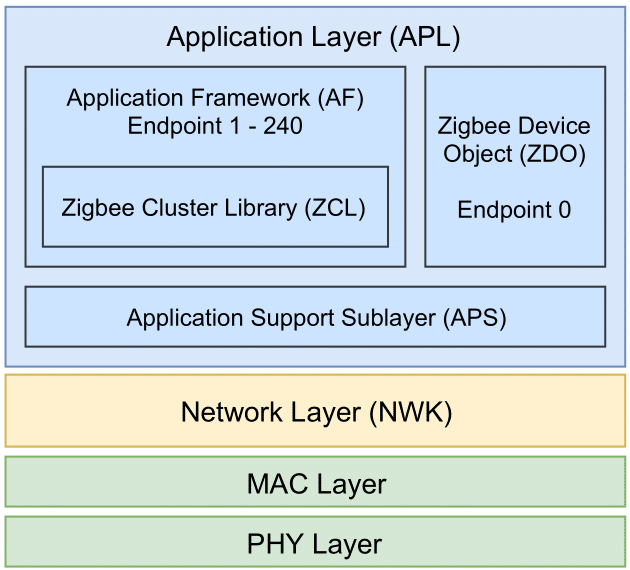
\includegraphics[width=\textwidth]{Zigbee_Architektur.png}
	\caption{Architektur des Zigbee Protokoll Stacks}
	\label{fig:ArchitekturdesZigbeeProtokollStacks}
\end{figure}

\subsection{Zigbee Software Development Kit}\label{subsec:ZigbeeSoftwareDevelopmentKit}
\todo[inline]{Eingesetzte SDK und deren Aufbau beschreiben. Allenfalls die wichtigsten API Funktionen genauer erläutern.}
